\chapter{Конструкторская часть}

В данной части будут разработаны функциональные схемы разрабатываемого ПО, а также разработаны структуры и алгоритмы, которые будут использованы в ПО.

\section{Функциональные схемы} 

На рисунках \ref{fig:A0} -- \ref{fig:A3} представлено формальное описании разрабатываемого ПО в виде idef0-диаграммы.

\begin{figure}[H]
	\centering
	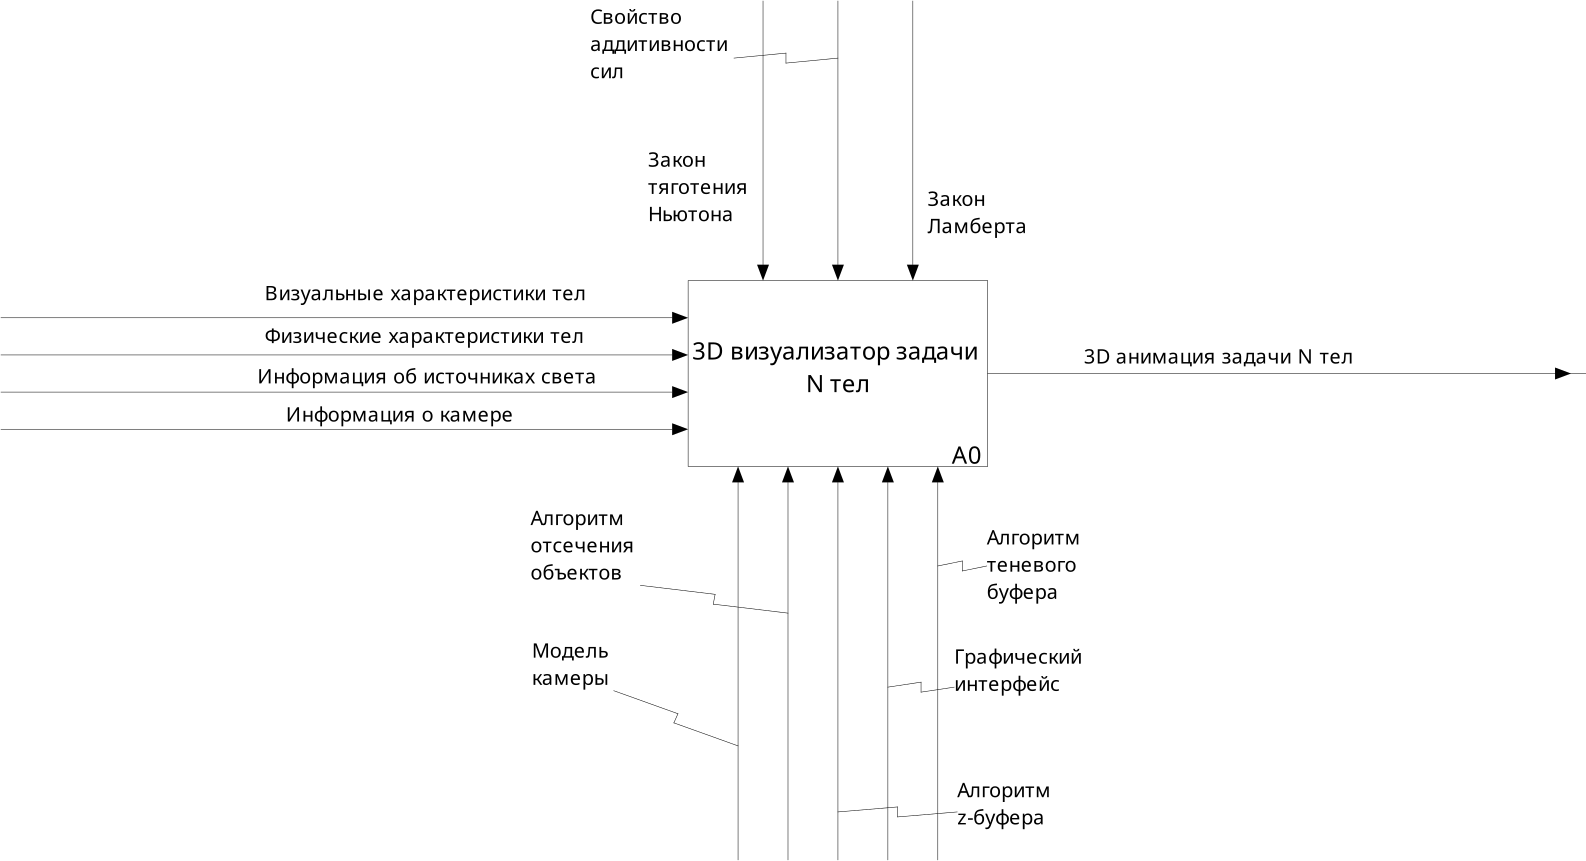
\includegraphics[width=0.9\textwidth]{ramus/01_A0}
	\caption{"Контекстная диаграмма верхнего уровня"}
	\label{fig:A0}
\end{figure}

\begin{figure}[H]
	\centering
	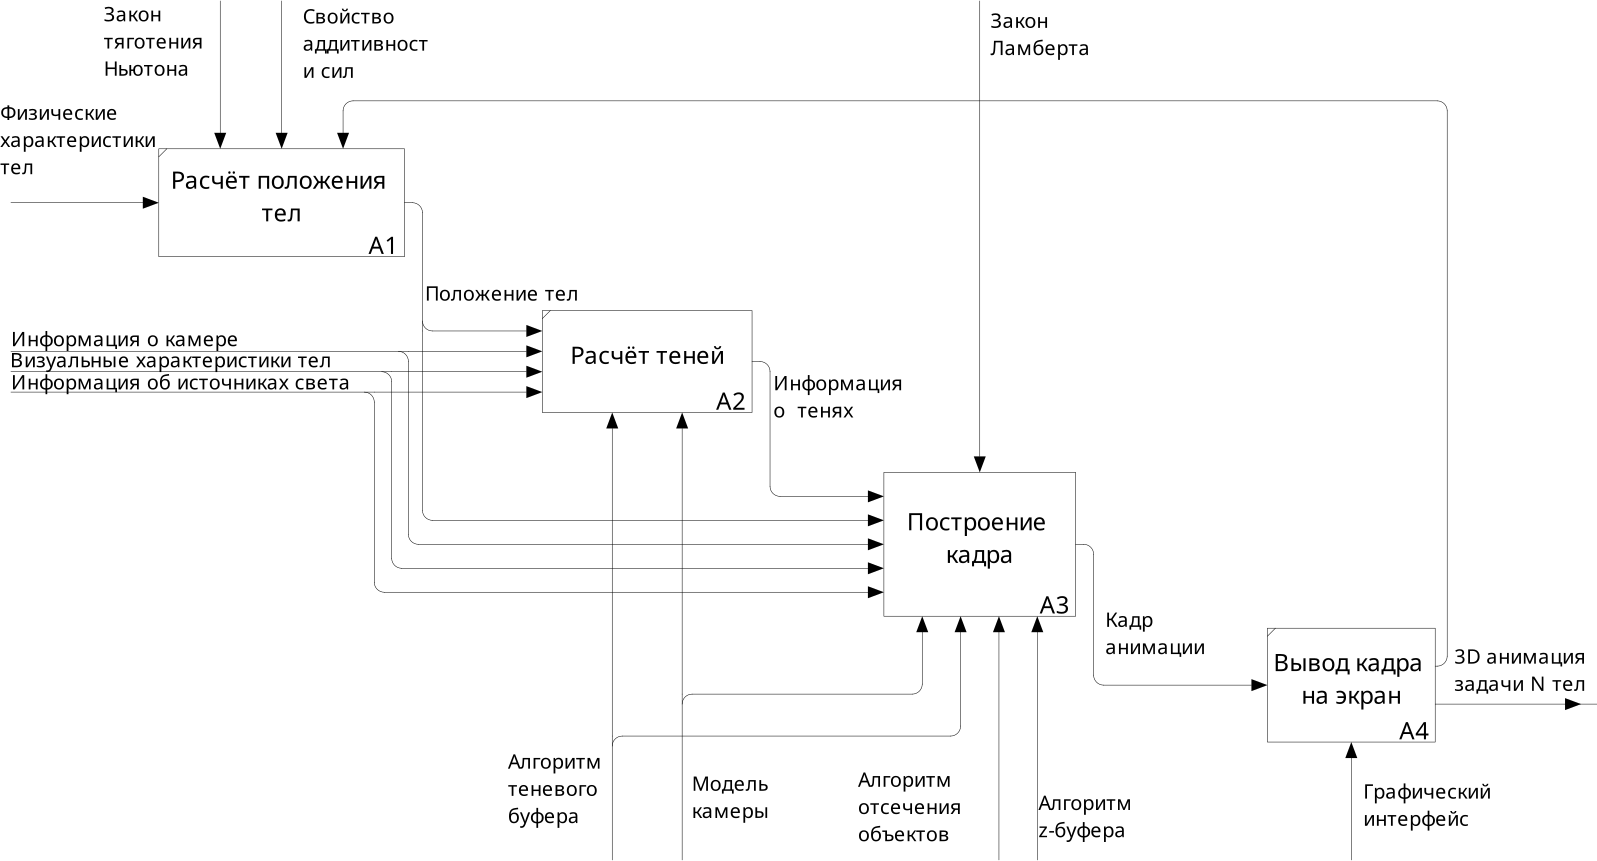
\includegraphics[width=0.9\textwidth]{ramus/02_A0}
	\caption{"Основной цикл ПО"}
	\label{fig:A1}
\end{figure}

\begin{figure}[H]
	\centering
	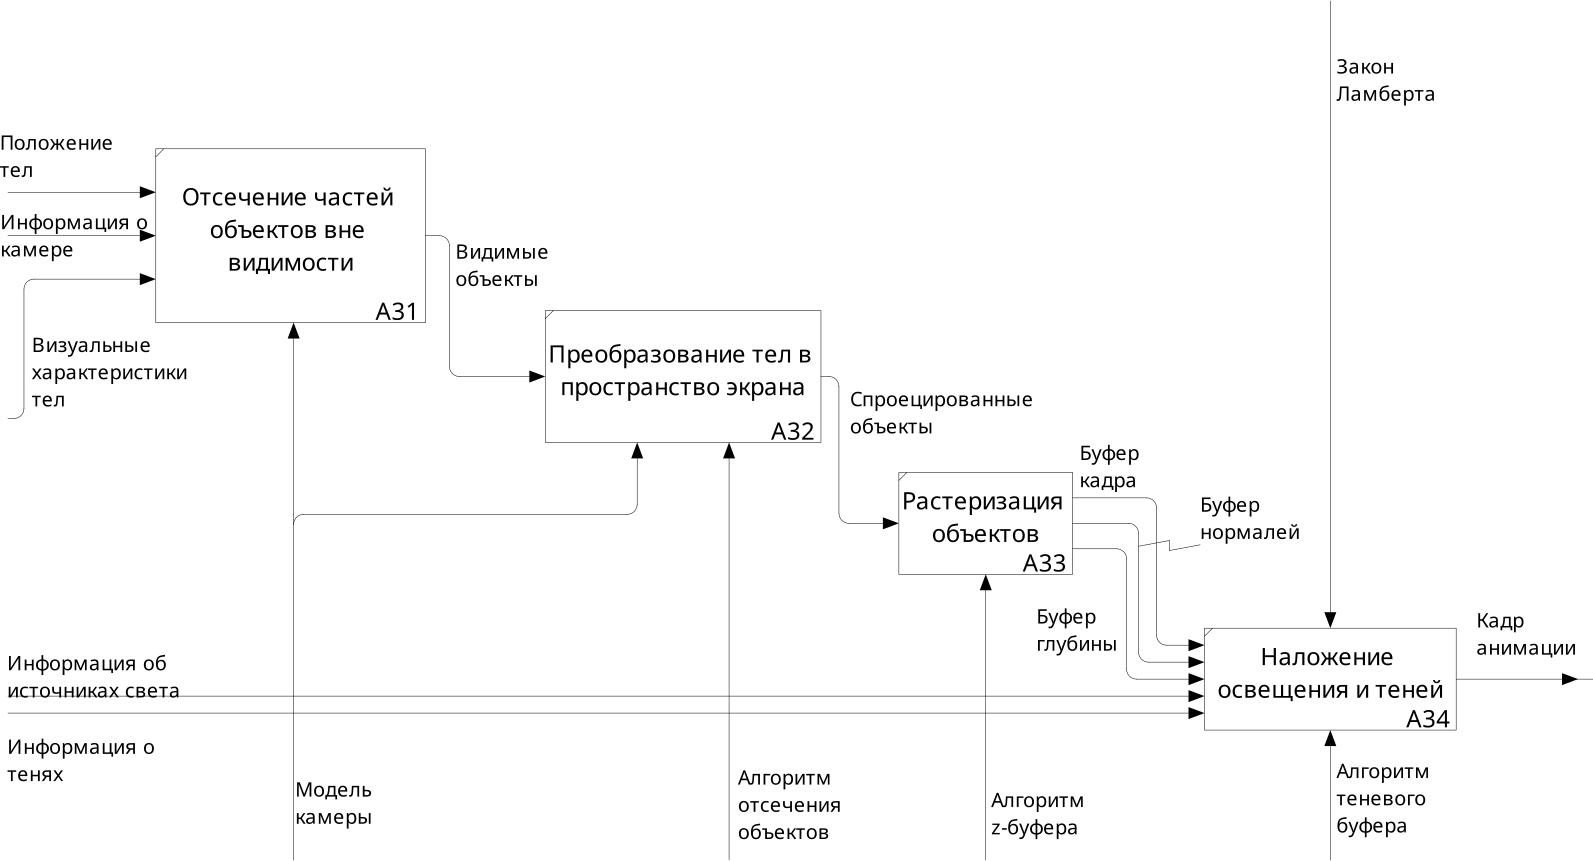
\includegraphics[width=0.9\textwidth]{ramus/03_A3}
	\caption{"Построение кадра"}
	\label{fig:A3}
\end{figure}

\section{Модель камеры}

Камера задаётся своим положением, направлением взгляда и направлением вверх и пирамидой видимости. Вектор в сторону получается векторным произведением вектора взгляда на вектор вверх. В пространстве камеры направление взгляда совпадает с положительным направлением оси z, а направление вверх -- с положительным направлением оси y.


Пирамида видимости -- усечённая 4-х гранная пирамида, уходящая в бесконечность, основание которой параллельно XoY. Основание пирамиды задаётся 3-мя параметрами:

\begin{itemize}
	\item $d$ -- расстояние от положения камеры до основания;
	\item $rx$ -- ширина основания;
	\item $ry$ -- высота основания.
\end{itemize}

Пирамида видимости в пространстве камеры продемонстрирована на рисунке \ref{fig:camera}.

\begin{figure}[H]
	\centering
	\includegraphics[width=0.5\textwidth]{camera}
	\caption{"Пирамида видимости камеры"}
	\label{fig:camera}
\end{figure}

Перспективная проекция по пирамиде видимости рассчитывается по формуле \ref{eq:perspective} \cite{projection}.

\begin{equation}
	\label{eq:perspective}
	\begin{pmatrix}
		x_p \\
		y_p \\
		z_p \\
		w_p \\
	\end{pmatrix} = 
	\begin{pmatrix}
		\frac{d}{rx}  & 0 & 0 & 0 \\
		0 & \frac{d}{ry} & 0 & 0 \\
		0 & 0 & 1 & 2d \\
		0 & 0 & 1 & 0 \\
	\end{pmatrix}
	\begin{pmatrix}
		x \\
		y \\
		z \\
		w \\
	\end{pmatrix}.
\end{equation}

Преобразование к пространству камеры выполняется по формуле \ref{eq:view} \cite{view}.

\begin{equation}
	\label{eq:view}
	\begin{pmatrix}
		x_v \\
		y_v \\
		z_v \\
		w_v \\
	\end{pmatrix} = 
	\begin{pmatrix}
		lx & ux & fx & 0 \\
		ly & uy & fy & 0 \\
		lz & uz & fz & 0 \\
		0 & 0 & 0 & 1 \\
	\end{pmatrix}
	\begin{pmatrix}
		x \\
		y \\
		z \\
		w \\
	\end{pmatrix},
\end{equation}
где
\begin{itemize}
	\item $\vec{u} = (ux, uy, uz)^T$ -- вектор взгляда;
	\item $\vec{f} = (fx, fy, fz)^T$ -- вектор вверх;
	\item $\vec{l} = (lx, ly, lz)^T = [\vec{u}, \vec{f}]$ -- вектор влево;
\end{itemize}


\section{Разработка алгоритма расчёта положения тел}

\textbf{Алгоритм расчёта положения тел}

\textbf{Входные данные:}
\begin{itemize}
	\item Массив тел $arr$, каждый элемент которого задан:
	\begin{itemize}
		\item $pos$ -- точка положения тела;
		\item $vel$ -- вектор скорости тела;
		\item $mass$ -- масса тела;
	\end{itemize}
	\item Размер массива $n$;
	\item Промежуток времени $dt$
\end{itemize}

\textbf{Выходные данные:}
\begin{itemize}
	\item Массив обновлённых тел $out\_arr$.
\end{itemize}

\textbf{Алгоритм}
\begin{itemize}
	\item создать пустой массив тел $out\_arr$ размера n;
	\item для каждого тела $body$ из массива $arr$:
	\begin{itemize}
		\item $dp = $ произведение вектора $vel$ на скаляр $dt$;
		\item $npos = pos + dp$
		\item $force = $ нулевой вектор;
		\item для каждого тела $infl$ из массива $arr$:
		\begin{itemize}
			\item если $infl$ не равен $body$:
			\item прибавить к $force$ силу действующую на  $body$ телом $infl$;
		\end{itemize}
		\item $nvel = vel + $ скалярное произведение $force$ на $\frac{dt}{mass}$;
		\item $nbody$ -- новое тело с параметрами ($npos$, $nvel$, $mass$);
		\item добавить $nbody$ в $out_arr$;
	\end{itemize}
	\item возврат $out\_arr$.
\end{itemize}

\textbf{Алгоритм расчёта силы, действующей одним телом на другое}
\textbf{Входные данные:}
\begin{itemize}
	\item $body$ -- тело, на которое действует сила;
	\item $infl$ -- тело, которое действует на $body$;
	\item каждое тело задано:
	\begin{itemize}
		\item $pos$ -- точка положения тела;
		\item $vel$ -- вектор скорости тела;
		\item $mass$ -- масса тела;
	\end{itemize}
\end{itemize}

\textbf{Выходные данные:}
\begin{itemize}
	\item $force$ -- вектор силы, действующий на $body$ со стороны $infl$.
\end{itemize}

\textbf{Алгоритм}

\begin{itemize}
	\item вектор $diff$ -- разность векторов $infl.pos$ и $body.pos$;
	\item $distance$ -- квадрат расстояние между $body$ и $infl$ -- $diff^2$;
	\item $force$ -- нормализованный вектор $diff$;
	\item умножить $force$ на скаляр $G=6.67430e^{-11} * infl.mass * body.mass / distance$;
	\item возврат $force$.
\end{itemize}

\section{Разработка алгоритма отсечения частей вне видимости камеры}

\textbf{Алгоритм отсечения нелицевых граней}

\textbf{Входные данные:}
\begin{itemize}
	\item $camera$ -- камера, заданная:
	\begin{itemize}
		\item $pos$ -- точка положения камеры;
		\item $forward$ -- вектор взгляда;
		\item $up$ -- вектор вверх;
		\item $px$ -- ширина окна камеры;
		\item $py$ -- высота окна камеры;
		\item $d$ -- расстояние до окна камеры;
	\end{itemize}
	\item $obj$ -- полигональный объект, заданный:
	\begin{itemize}
		\item $vertices$ -- массив точек;
		\item $polygons$ -- массив полигонов, каждый из которых задан 3-мя точками из массива $vertices$ -- $v1$, $v2$, $v3$ и вектором внутренней нормали $normal$.
	\end{itemize}
\end{itemize}

\textbf{Выходные данные:}
\begin{itemize}
	\item $nobj$ -- полигональный объект без нелицевых граней.
\end{itemize}

\textbf{Алгоритм}

\begin{itemize}
	\item создать пустой массив полигонов $npolygons$ размером массива $polygons$;
	\item для каждого полигона $poly$ из массива $polygons$:
	\begin{itemize}
		\item если скалярное произведение $poly.normal$ и $camera.forward$ > 0:
		\item добавить $poly$ в массив $npolygons$
	\end{itemize}
	\item создать пустой массив точек $nvertices$ размером массива $vertices$;
	\item для каждого полигона $npoly$ из массива $npolygons$:
	\begin{itemize}
		\item добавить $npoly.v1$, $npoly.v2$, $npoly.v3$ в массив $nvertices$;
	\end{itemize}
	\item создать полигональный объект $nobj$ c $nvertices$ и $npolygons$;
	\item вернуть $nobj$.
\end{itemize}

\textbf{Алгоритм отсечения частей объектов вне поля видимости камеры}

При отсечении по зоне видимости используются плоскости, образующие пирамиду видимости. Каждая такая плоскость описывается парой: внутренняя нормаль и скалярное значение. Методом, описанном в \cite{gabriella}, были найдены плоскости для используемой модели камеры:

\begin{itemize}
	
\begin{itemize}
	\item задняя -- $((0, 0, 1), -d)$
	\item левая -- $((\frac{2d}{px}, 0, 0), 0)$
	\item задняя -- $((0, 0, 1), -d)$
	\item задняя -- $((0, 0, 1), -d)$
	\item задняя -- $((0, 0, 1), -d)$
\end{itemize}  

\textbf{Входные данные:}
\begin{itemize}
	\item $camera$ -- камера, заданная:
	\begin{itemize}
		\item $pos$ -- точка положения камеры;
		\item $forward$ -- вектор взгляда;
		\item $up$ -- вектор вверх;
		\item $px$ -- ширина окна камеры;
		\item $py$ -- высота окна камеры;
		\item $d$ -- расстояние до окна камеры;
	\end{itemize}
	\item $obj$ -- полигональный объект, заданный:
	\begin{itemize}
		\item $vertices$ -- массив точек;
		\item $polygons$ -- массив полигонов, каждый из которых задан 3-мя точками из массива $vertices$ -- $v1$, $v2$, $v3$ и вектором внутренней нормали $normal$.
	\end{itemize}
\end{itemize}

\textbf{Выходные данные:}
\begin{itemize}
	\item $nobj$ -- полигональный объект без невидимых частей.
\end{itemize}

\textbf{Алгоритм}

\begin{itemize}
	\item преобразовать $obj$ в пространство камеры;
	\item
	\item создать пустой массив полигонов $npolygons$ размером массива $polygons$;
	\item 
\end{itemize}


\section{Разработка алгоритма z-буфера}

\section{Разработка алгоритма теневого буфера}


\section*{Вывод}

\clearpage
